\chapter{Fluid Simulation}\label{chapter:fluid-simulation}
Simulating convincing fluid dynamics is a continuing challenge of computer
graphics, especially when considering real-time applications. There are multiple
established ways to simulate fluids, the most widespread being Eulerian (i.e.
grid-based) and Lagrangian (i.e. particle-based) methods. Here, we restrict
ourselves to discussing Eulerian methods, and also introduce the Laplacian
Eigenfunction method (\cite{dewitt}).

The dynamics of fluids are governed by the Navier-Stokes Equations:
\begin{equation}\label{eq:NSE}
    \pdv{\vb{u}}{t} + (\vb{u}\cdot\grad)\vb{u}
    = -\frac{1}{\rho}\grad{p} + \nu\grad^2\vb{u} + \vb{f},
\end{equation}

where $\vb{u}$ is the velocity of the fluid, $\rho$ is the density, $p$ is the
scalar pressure field, $\nu$ is the viscosity constant, and $\vb{f}$ denotes
external forces. For incompressible fluids, the divergence-freeness also has to
hold, i.e. $\div{\vb{u}} = 0$

Even though equation~\eqref{eq:NSE} already describes the evolution of the fluid
as a \acf{PDE}, it is too complex for simply stepping it forward in time with
Euler steps. Instead, a technique called \textit{operator splitting} is applied
for numerical simulations, where each term is treated individually, and their
effect is combined together to fully approximate the original equation. We give
a short overview of each term to get a general understanding of fluid
simulation, first treating the problem in an Eulerian way (i.e.  sampling
$\vb{u}$ on a grid), building up our way towards the Laplacian Eigenfunction
method discussed in section~\ref{section:laplacian-eigenfluids}.  For a more
complete overview of established fluid simulation techniques, see
\cite{FluidNotes} and \cite{BridsonFluid}.

Equation~\eqref{eq:NSE} is usually split by separating out the advection part,
the external force part, and the pressure/incompressibility part. When viscosity
is important, that can also be separated. This means, we work out methods for
solving these simpler equations:
\begin{align*}
    \dv{q}{t} &= 0              \qq{(advection)}\\
    \pdv{\vb{u}}{t} &= \vb{p}   \qq{(external forces)}\\
    \pdv{\vb{u}}{t} + \frac{1}{\rho}\grad p &= 0 \\
    \qq{such that}\div{\vb{u}} &= 0.
                                \qq{(pressure, enforcing incompressibility)}
\end{align*}

A generic quantity $q$ is used in the advection equation, because as we also
show later on in our experiments, we may be interested in advecting other field
quantities than just the velocity $\vb{u}$. For the advection part, we develop
an algorithm called $\text{Advect}(\vb{u}, \Delta t, q)$: it advects quantity
$q$ through the velocity field $\vb{u}$ for a time interval $\Delta t$. 

For the external forces, any traditional numerical integration approach, such as
forward Euler can be used: $\vb{u}^{t+1} = \vb{u}^t + \Delta t \vb{f}$.

For calculating the pressure, an algorithm $\text{Project}(\Delta t, \vb{u})$
calculates and applies just the right amount of pressure to the velocity field
to make it divergence-free, and also enforce any solid wall boundary
conditions. The term "project" comes from the fact that the algorithm
essentially projects $\vb{u}$ to the closest divergence-free velocity field, and
interpreting the difference between these two fields as a pressure resulting
from "particles" being too close together. 

The order in which these algorithms are being applied matters a lot, as the
advection must be done on a divergence-free field, which means the output of
$Project$. Putting all of these together, we arrive at a basic fluid simulation
algorithm:

\begin{algorithmic}
    \State $\vb{u}^0 \gets \text{an initial divergence-free velocity field}$
    \For{$t = 0, 1, 2 \dots $}
        \State $\Delta t 
            \gets \text{a suitable timestep to go from $t_n$ to $t_{n+1}$}$
        \State $\widetilde{\vb{u}} 
            \gets \text{Advect}(\vb{u}^n,\Delta t, \vb{u}^n)$
        \State $\widetilde{\vb{u}} 
            \gets \widetilde{\vb{u}}^n + \Delta t \vb{f}$
        \State $\vb{u}^{n+1}
            \gets \text{Project}(\vb{u}^n,\Delta t, \vb{u}^n)$
            \EndFor \Comment{$[\vb{u}^0, \dots, \vb{u}^t]$ is the simulated
            fluid flow for $t$ timesteps.}
\end{algorithmic}

\todo{Semi-Lagrangian Advection. It is trivial in a Lagrangian setting...}

\todo{For our smoke simulation examples, we are using a MacCormak advection
scheme that uses a forward as well as a backward lookup to estimate and correct
the error of the semi-langrangian advection.}

\todo{Making fluids incompressible via pressure projection: $\vb{u}^{n+1}
= \vb{u} - \Delta t \frac{1}{\rho} \grad p$, with $\div{\vb{u}^{n+1}} = 0$. Look
up, and include which one we are using.}

\todo{Projecting a velocity field involvess solving for the pressure, and
subtracting its spatial gradient.}

\section{The Laplacian Eigenfunction Method}
\label{section:laplacian-eigenfluids}

\todo{Finish writing this section.}

\cite{dewitt} introduced the method of using Laplacian eigenfunctions for fluid
simulation. \cite{scalable-eigenfluids} addressed scalability and generalization
issues, and referred to the technique as eigenfluids. 

The main idea is to express the velocity field $\vb{u}(\vb{x})$ via the linear
combination of $N$ global functions:

\begin{equation}\ref{eq:u-lin-comb}
\vb{u}(\vb{x})=\sum_i^N w_i \Phi_i(\vb{x}),
\end{equation}

where the elements of $\vb{w} = [w_0, \dots, w_N]$, are called \textit{basis
coefficients}, and ${\Phi_i}$ are \textit{basis functions}.

As our basis functions, we choose the eigenfunctions of the vector Laplacian
operator $\Delta = \grad^2 = \text{grad}(\text{div}) - \text{curl}^2$, which
further simplifies to $\grad^2 = -\text{curl}^2$ for divergence-free fields (see
section~\ref{section:vector-laplacian}). 

Besides being eigenfunctions of the vector Laplacian operator, if we further
require our basis fields $\Phi_{\vb{k}}$ to be divergence-free, and to satisfy
a free-slip boundary condition, our basis functions are fully characterized by
\begin{align*}
\nabla^2 \Phi_{\textbf{k}} &= \lambda_{\textbf{k}}\Phi_{\textbf{k}} \\
\nabla \cdot \Phi_{\textbf{k}} &= 0 \\
\Phi_{\textbf{k}} \cdot \textbf{n} &= 0 \text{ at } \partial D,
\end{align*}
where $\textbf{n}$ is the normal vector at boundary $\partial D$.

Closed-form expressions of $\Phi_{\vb{k}}$ exist on the two dimensional $D \in
[0, \pi] \times [0, \pi]$ square domain (\cite{chengfield}). Notating the two
scalar components in the x and y directions $\Phi_{\vb{k}} =(\Phi_{\vb{k}, x},
\Phi_{\vb{k},y})$, we can write them as
\begin{align*}\label{eq:explicit-u}\numberthis
    \Phi_{\vb{k},x}(x, y) &= \eta_{\vb{k}}
    ( k_2 \sin(k_1 x) \cos(k_2 y) ) \\
    \Phi_{\vb{k},y}(x, y) &= -\eta_{\vb{k}}
    ( -k_1 \cos(k_1 x) \sin(k_2 y) ),
\end{align*}

where $\vb{k} = (k_1, k_2) \in \mathbb{Z}^2$ is the \textit{vector wave number},
$\lambda_{\vb{k}} = -(k_1^2 + k_2^2)$ is the eigenvalue, and $\eta_{\vb{k}}
= \frac{1}{-\lambda_{\vb{k}}} = \frac{1}{k_1^2 + k_2^2}$ is a normalization
parameter.  \cite{scalable-eigenfluids} use $\frac{1}{\sqrt{-\lambda}}
= \frac{1}{\sqrt{k_1^2 + k_2^2}}$ for normalization, but we keep the non-root
version, as we did not notice any subtantial difference between the two during
implementation.

As an example, $\Phi_{4,3}(x,y)$ is visualized on figure~\ref{fig:phi-example}.
In appendix~\ref{appendix:first_16}, we also plot the first $16$ basis fields.

\begin{figure}
  \centering
  \begin{subfigure}[t]{0.48\textwidth}
    \centering
    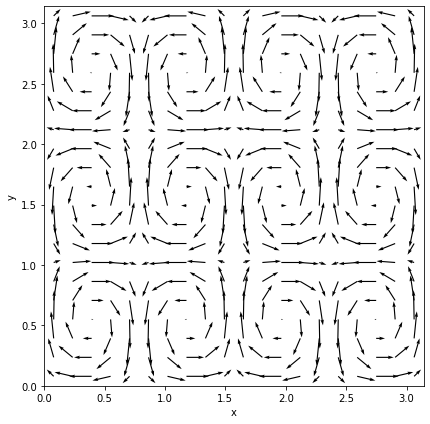
\includegraphics[height=\textwidth]{figures/eigenfluids/k_4_3_vel.png}
    \caption{Velocity field $\Phi_{4,3}$.}
  \end{subfigure}
  \begin{subfigure}[t]{0.48\textwidth}
    \centering
    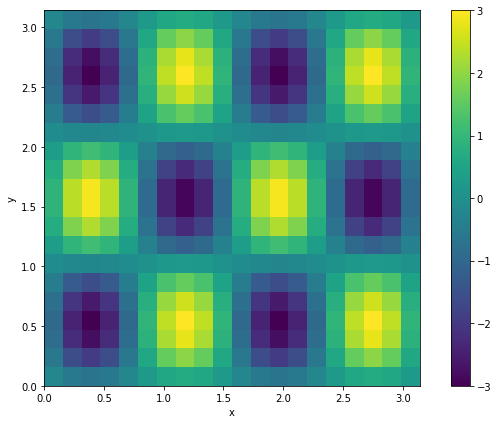
\includegraphics[height=\textwidth]{figures/eigenfluids/k_4_3_curl_bar.png}
    \caption{Curl field $\curl{\Phi_{4,3}} = \phi_{4,3}$.}
  \end{subfigure}\par\medskip
  \caption{Visualizing $\Phi_{4,3}$ sampled on a $20 \times 20$ grid in
  our simulation domain $D = [0,\pi] \times [0,\pi]$.}
  \label{fig:phi-example}
\end{figure}

\subsection*{Vorticity Basis Fields}
Taking the curl of the velocity basis fields $\Phi_{\vb{k}}$ gives us the
vorticity fields (as introduced in section~\ref{section:curl}):
\begin{align*}
    \phi_{\vb{k}} &= \curl{\Phi_{\vb{k}}} 
    =  \pdv{\Phi_{\vb{k},y}}{x} - \pdv{\Phi_{\vb{k},x}}{y}\\
&= -\mu_{\vb{k}} k_1 \sin(k_2 y) k_1(-sin(k_1 x)) - \mu_{\vb{k}} k_2 \sin(k_1 x)
    k_2 (-sin(k_2 y))\\
&= \mu_{\vb{k}} sin(k_1 x) sin(k_2 y)(k_1^2+k_2^2) = sin(k_1 x) sin(k_2 y)
\end{align*}
Interpreting this as the third component of a 3D vector,
$$\phi_{\vb{k}} = \curl{\Phi_{\vb{k}}} 
= \mqty(0 \\ 0 \\ \sin(k_1 x) \sin(k_2 y)).$$

\todo{We defined the curl in the mathematical foundations chapter as being
scalar. We have to mention it there that the 2D curl can also be defined a 3D
vector, with the 3rd component being the only non-negative value.}

\subsection*{Dynamics}

\todo{Write this section}

The vorticity formulation of the Navier-Stokes equation is
\begin{equation}\label{eq:NSE-vorticity}
    \dot{\bf{\omega}} = \text{Advect}(\bf{u}, \bf{\omega}) + \nu \Delta\bf{\omega}
    + \text{curl}(\bf{f}),
\end{equation}
where $\bf{\omega} = \curl{\bf{u}}$ and $\bf{f}$ are external forces.

\subsection*{Advection}
The Advect$(\Phi_i, \phi_j)$ term represents the non-linear advection of basis
fields. We precompute these, and the vorticity basis coefficients of the results
are stored in ``a set of $\vb{C}_k$ matrices'' (\cite{dewitt}, resulting in $N$
number of $N \times N$ matrices), or equivalently, a ``$3^{rd}$ order advection
tensor $\mathfrak{C}$'' (\cite{scalable-eigenfluids}).  The dimensions of
$\vb{C}$ and $\mathfrak{C}$ are both $N \times N \times N$. We will refer to
these precomputed advection values as $N$ $\vb{C}_k$ matrices.
The respective works also propose different ways to precompute these values:

\cite{dewitt}:

\begin{equation}\label{eq:Ck-dewitt}
\vb{C}_g[h, i] = \Big( \curl(\phi_h \cross \Phi_i)\Big)\cdot \phi_g
\end{equation}

\cite{scalable-eigenfluids} improves on \eqref{eq:Ck-dewitt} by using the method
introduced by \cite{ModelReductionFluidSim}:
\begin{equation}
    \mathfrak{C}(g,h,i) = \int_D (\curl{\Phi_i})\cdot (\Phi_g \cross \Phi_h)
    \text{d}D,
\end{equation}
noting improvements such as preserving the anti-symmetry of the tensor by
construction, i.e. $\mathfrak{C}(g,h,i) = -\mathfrak{C}(h,g,i)$. We keep with
calculating the advection coefficients in line with \eqref{eq:Ck-dewitt}, as it
was working well enough for our purposes of differentiable physics simulation.

\subsubsection*{Precalculating the Advection Matrices}
For finding the structure coefficients of the $\vb{C}_k$ matrices, we can start
from writing out the advection operator $\text{Advect}(\Phi_i, \phi_j)
= \curl(\phi_j \cross \Phi_i)$ as
\begin{align*}
\curl(\phi_j \cross \Phi_i) = \Big(
    &\frac{1}{\lambda_i}i_1j_2cos(i_1x)cos(j_2y)sin(j_1x)sin(i_2y)\\
    &-\frac{1}{\lambda_i}i_2j_1cos(j_1x)cos(i_2y)sin(i_1x)sin(j_2y)
\Big).
\end{align*}

\todo{See appendix for math details?}

The trigonometric identity $cos(\alpha)sin(\beta)
= \frac{1}{2}sin(\alpha+\beta)-\frac{1}{2}\sin(\alpha-\beta)$ enables factoring
to a suitable expression which is in the span of ${\phi_k}$:
\begin{align*}
\text{Advect}(\Phi_i,\phi_j)= \frac{1}{4\lambda_{i}}
    \Big[&(i_1 j_2 - i_2 j_1)\phi_{i_1+j_1, i_2+j_2}\\
     &-(i_1 j_2 + i_2 j_1)\phi_{i_1+j_1, i_2+j_2}\\
     &+(i_1 j_2 + i_2 j_1)\phi_{i_1-j_1, i_2+j_2}\\
     &-(i_1 j_2 - i_2 j_1)\phi_{i_1-j_1, i_2-j_2}\Big]\\
\end{align*}
The resulting coefficients are
\begin{align*}
    \vb{C}_{i_1+j_1,i_2+j_2}[i,j] &= -\frac{1}{4(i_1^2 + i_2^2)}(i_1j_2-i_2j_1)\\
    \vb{C}_{i_1+j_1,i_2-j_2}[i,j] &= -\frac{1}{4(i_1^2 + i_2^2)}(i_1j_2+i_2j_1)\\
    \vb{C}_{i_1-j_1,i_2+j_2}[i,j] &= -\frac{1}{4(i_1^2 + i_2^2)}(i_1j_2+i_2j_1)\\
    \vb{C}_{i_1-j_1,i_2-j_2}[i,j] &= -\frac{1}{4(i_1^2 + i_2^2)}(i_1j_2-i_2j_1).\\
\end{align*}

\textbf{Note:} We are using $\vb{k} = (k_x, k_y) = (k_1, k_2)$. A single
(non-vector) $k$ is also used for indexing over all of the basis fields --
a slight, but very useful abuse of notation, stemming from the fact that
a suitable remapping from vector wave lengths $(k_1, k_2)$ to positive integers
is necessary in an implementation.

\todo{I didn't come across any alternative naming convention to denote the
advection, that is not a function named with a whole word.}



















